\documentclass{article}
\usepackage[margin=3.5cm]{geometry}
\usepackage{pdfpages}
\usepackage{graphicx}
\DeclareGraphicsExtensions{.pdf,.png,.jpg}	

\title{Homework III}
\author{Gregory Williams\\GW4975\\EE 382C Requirements Engineering}
\date{11/06/2015}

\begin{document}
	\maketitle
	
	\section*{Installation Requirements}
	\begin{itemize}
	\item 2 GHz processors\\
		The administrators expect faster computers.\\
	\item 2 GB memory\\
		The administrators expect more computational capability.\\
	\item support for gigabit networks
		The administrators expect faster and more robust network communication.\\
	\end{itemize}
	The hardware requirements change as better hardware becomes cheaper; better performance in systems is a constant want, if not need. Most local installations can expect the requirements for new hardware to increase with time.
	\section*{Non-Functional Requirements}
	\begin{itemize}
	\item "users expect no more than 2 seconds per transaction for all requests"\\
		This applies to the system's runtime performance. It may be evaluated by executing system functionality and measuring system responsiveness.\\
	\item "Federal regulations require payment data to be encrypted when transmitted or stored"\\
		This applies to the system's communication and data storage. It may be evaluated by grabbing dumps of databases or intercepting (sniffing) network communications of the system and ensuring the content is encrypted.\\
	\item "intention to extend the system with many additional services in the future"
		This applies to the system's architecture; an extensible framework must underpin the entire system so that it may be extended at a later date. This could be evaluated by having core pieces of the system implemented as modular plugins to some bare framework, bringing extensibility and demonstrative architecture to the system from the very beginning. If "registration" is a plugin, then it can be shown that additional functionality can be added later.\\
	\end{itemize}

	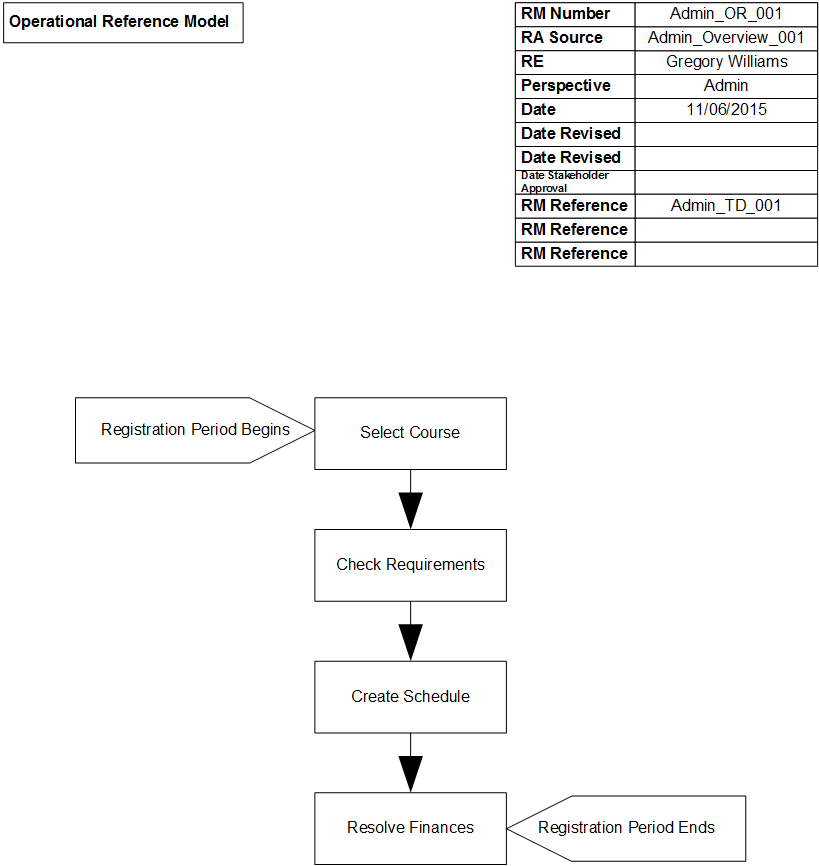
\includegraphics[width=\textwidth]{OperationalReferenceModel}
	\\
	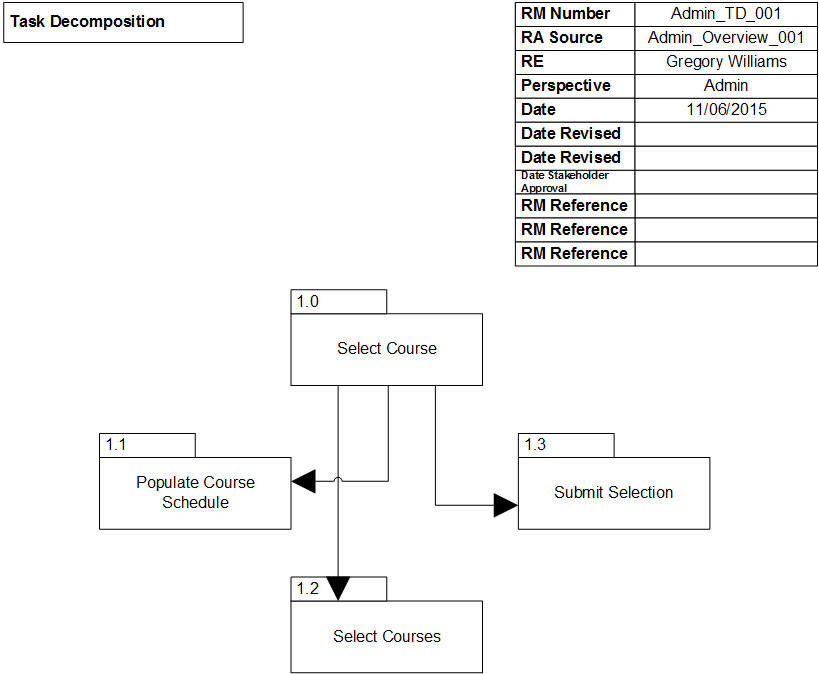
\includegraphics[width=\textwidth]{TaskDecomposition1}
	\\
	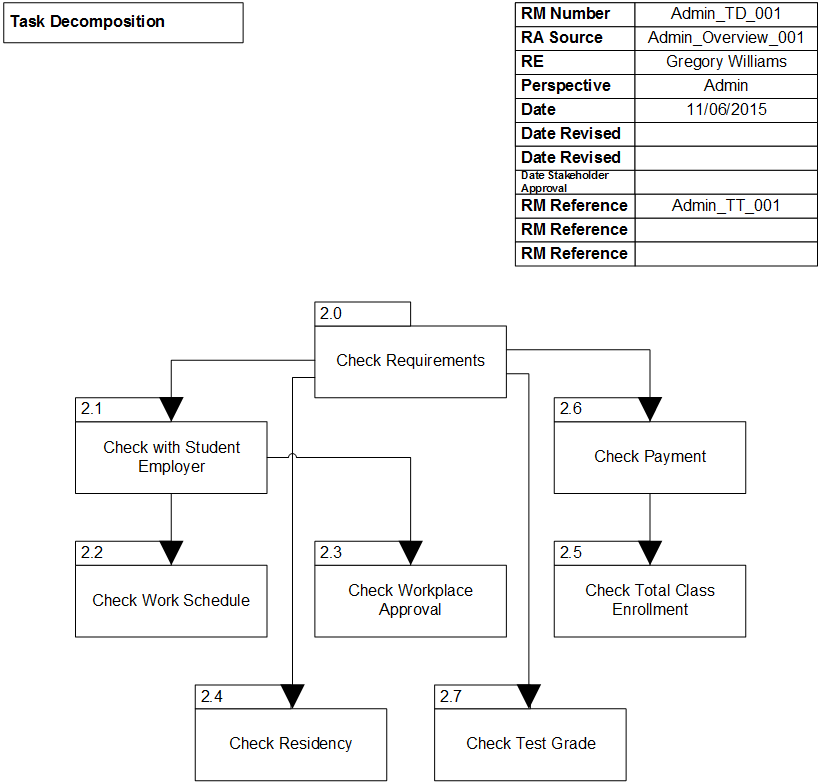
\includegraphics[width=\textwidth]{TaskDecomposition2}
	\\
	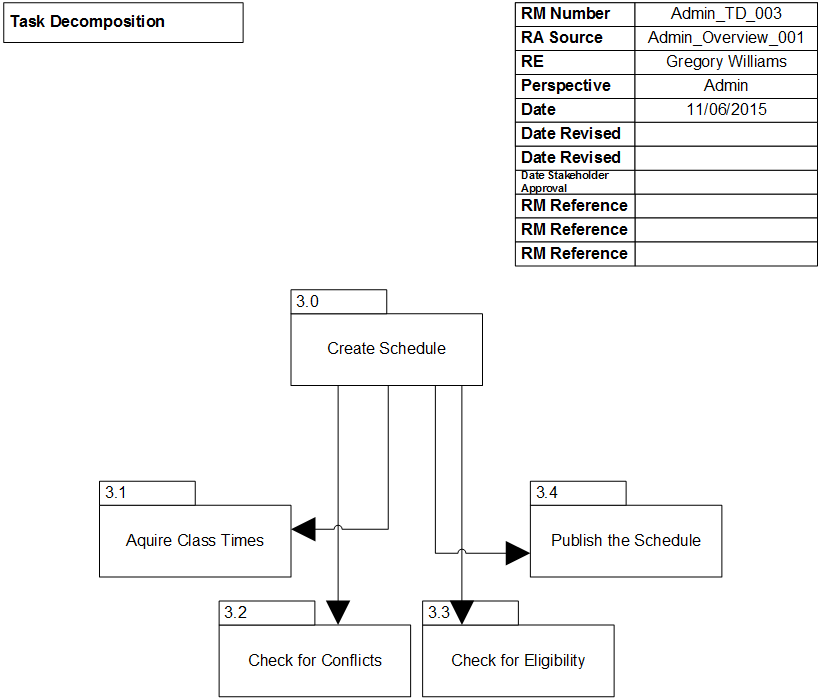
\includegraphics[width=\textwidth]{TaskDecomposition3}
	\\
	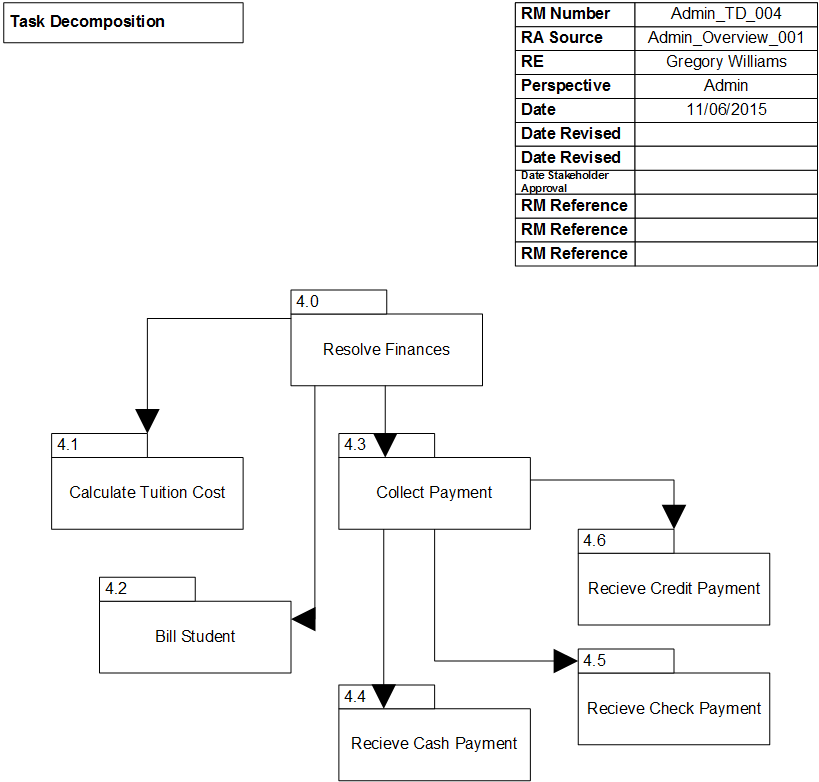
\includegraphics[width=\textwidth]{TaskDecomposition4}
	\\
	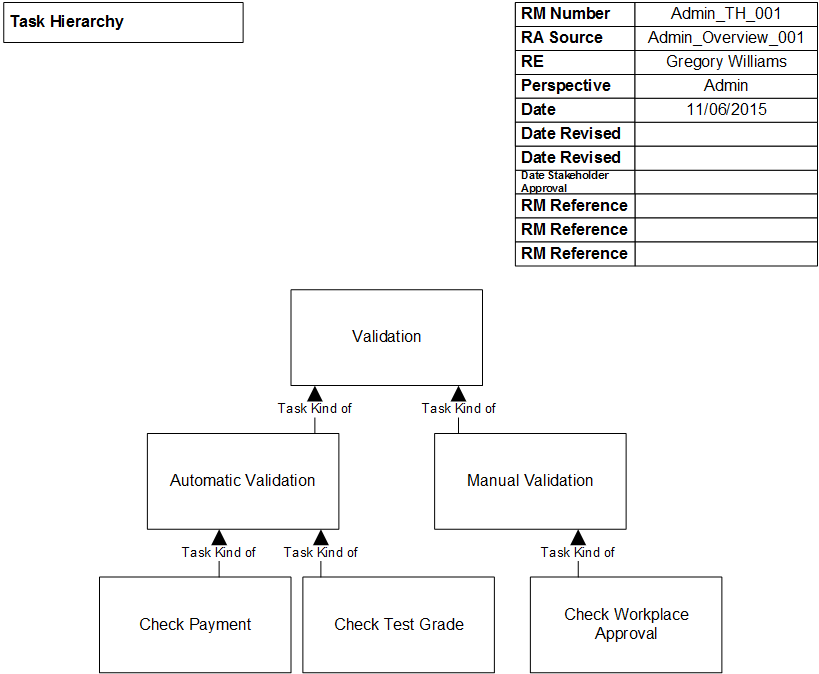
\includegraphics[width=\textwidth]{TaskHierarchy}
	\\

	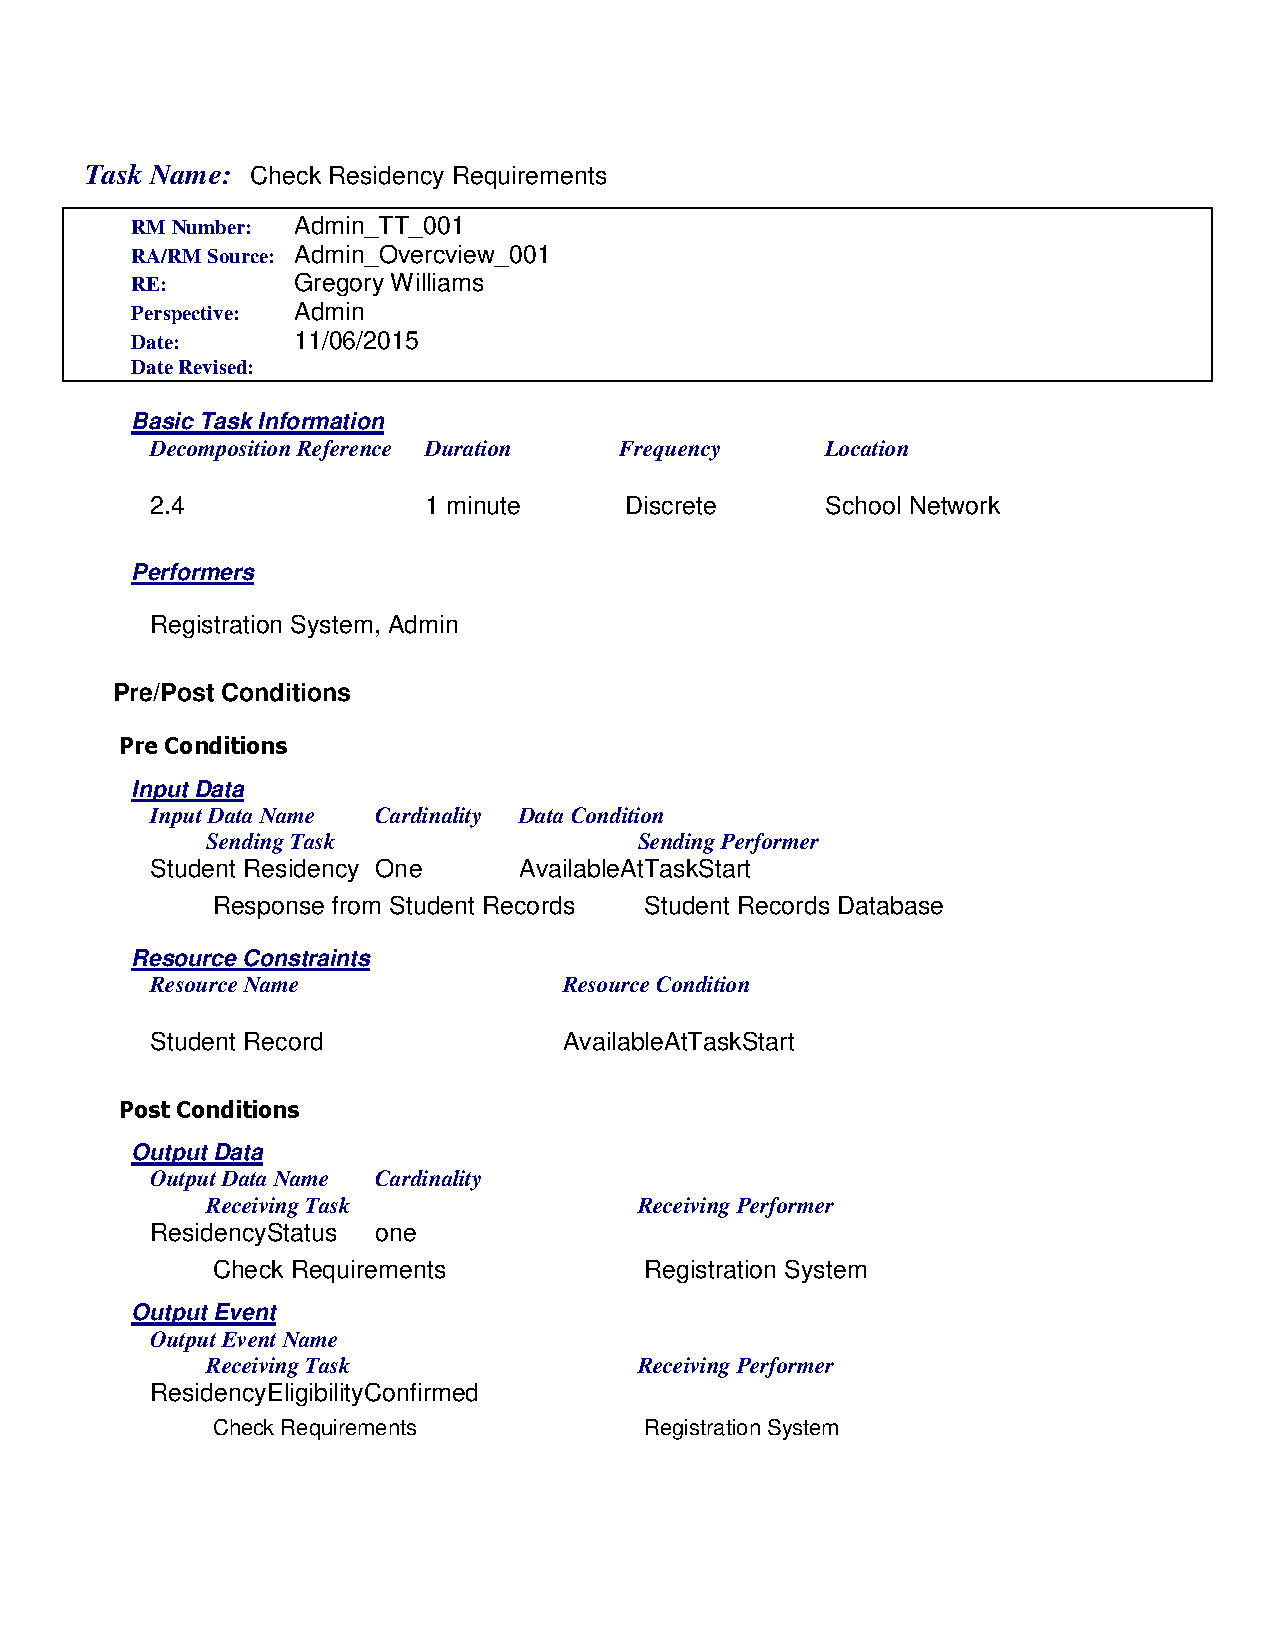
\includepdf[width=\textwidth,pages=-]{Task}
	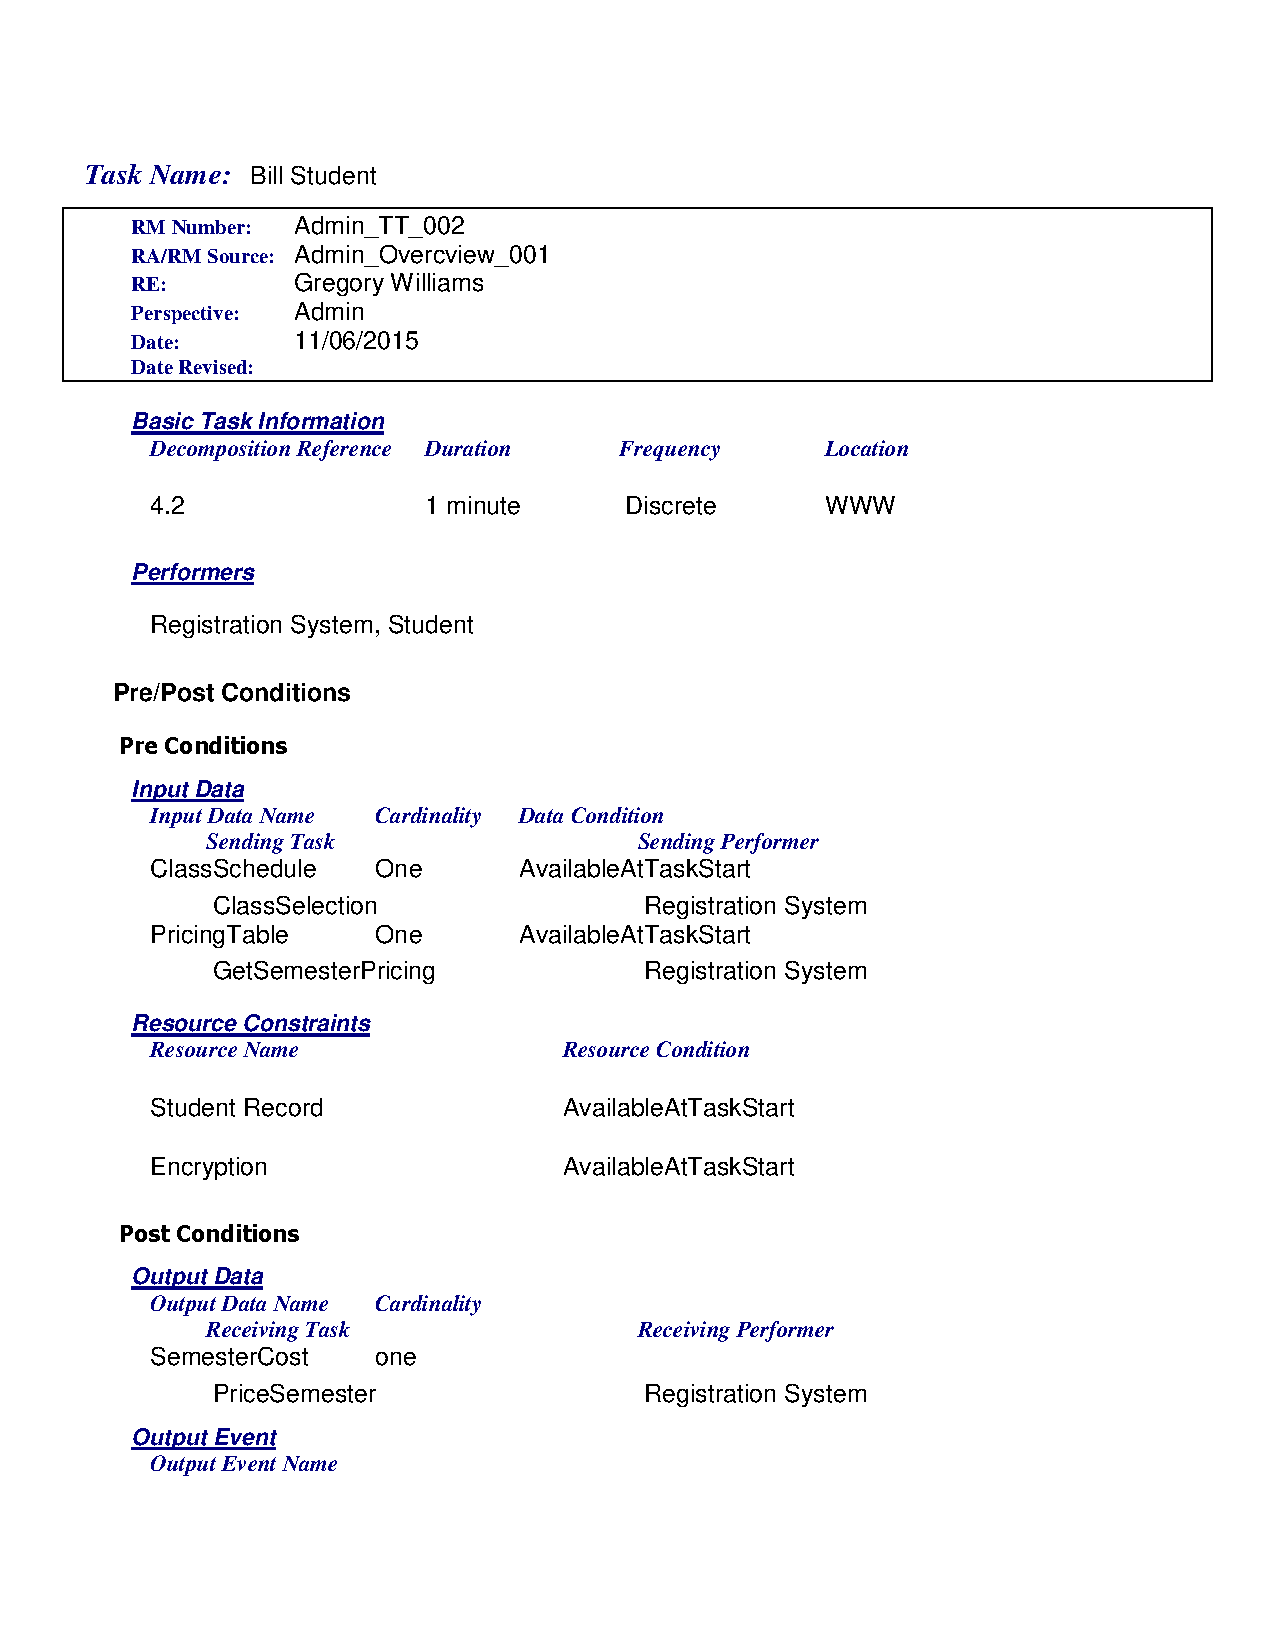
\includepdf[width=\textwidth,pages=-]{Task2}

	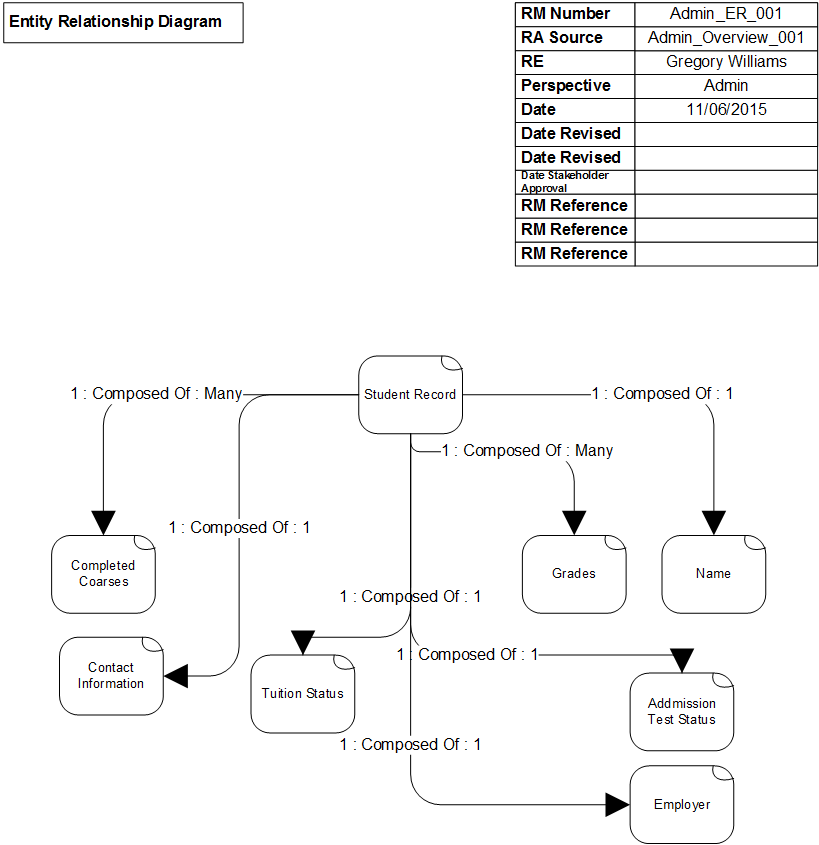
\includegraphics[width=\textwidth]{EntityRelationship}
	\\
	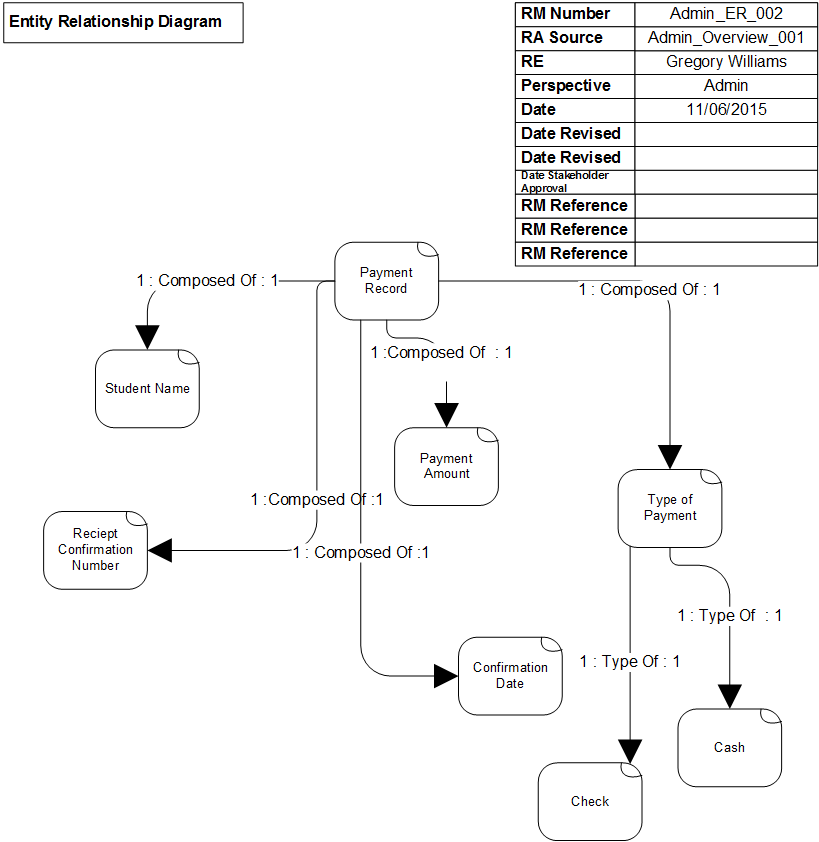
\includegraphics[width=\textwidth]{EntityRelationship2}
	\\
	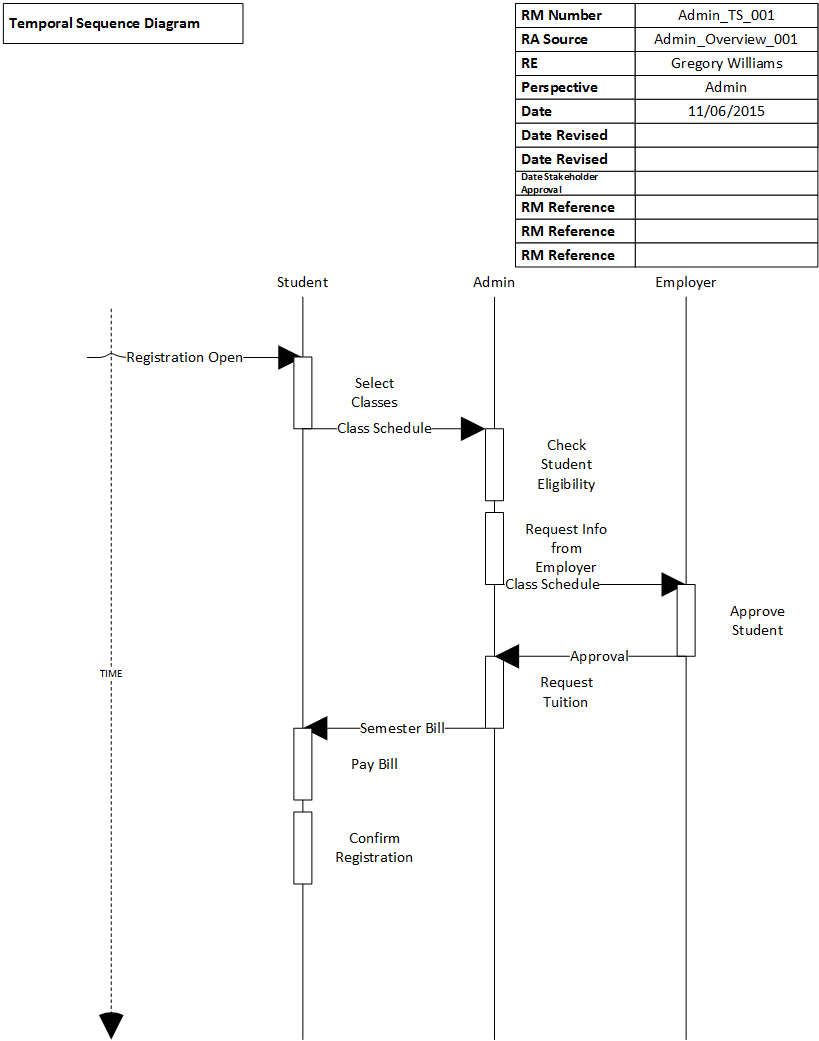
\includegraphics[width=\textwidth]{TemporalSequence}
	\\
	
	\section*{Inconsistent Requirements}
	The type of payment received by the system must support cash, check, or credit card. But the financial record can only hold check or cash. This inconsistency will have to be resolved when the representations are synthesized.
	\section*{Additional Acquirement Priorities}
	\begin{itemize}
	\item \texttt{Admin\_TD\_003}\\
		The Task Decomposition does not indicate any of the concrete requirements in how students and administrators will validate that the conflicts have indeed been resolved. I would want to follow up with the administration and with current students on their expectations for how the conflicts are communicated if they exists, and if there is any desired functionality or interaction expectations in both the no-conflict case and the conflict case.\\
	\item \texttt{Admin\_TS\_001}\\
		The Temporal Sequence Diagram does not include any information about what administrators need to do if/when the income constraint prevents a class from being offered that students are currently registered for. We would need to acquire the timing and task that administrators would take in the case that a class is canceled.\\
	\end{itemize}
\end{document}